\subsection{\bap and the Running Example}

\begin{figure}
\begin{minipage}[c]{.45\linewidth}
  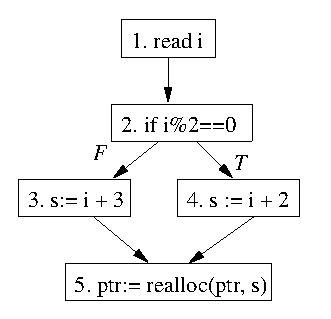
\includegraphics{fig/running-example}
  \label{vine:running-example-fig}
\end{minipage}
\begin{scriptsize}
\begin{minipage}[c]{.45\linewidth}
\begin{lstlisting}
// address instr dst, src
0x8048419 push   ebp  // setup stack
0x804841a mov    ebp,esp
0x804841c sub    esp, 0x18
0x804841f lea    eax, [ebp-0x8]
0x8048422 mov    [esp], eax 
0x8048425 call   0x80483f4 // call read
0x804842a mov    eax, [ebp-0x8]
0x804842d and    eax, 0x1  // if i%2==0
0x8048430 test   eax,eax
0x8048432 jne    0x804843f
0x8048434 mov    eax,[ebp-0x8]
0x8048437 add    eax, 0x2  // s := i+2
0x804843a mov    [ebp-0x4], eax
0x804843d jmp    0x8048448
0x804843f mov    eax,[ebp-0x8]
0x8048442 add    eax,0x3  // s := i+3
0x8048445 mov    [ebp-0x4], eax
0x8048448 mov    eax, [ebp-0x4]
0x804844b mov    [esp+0x4], eax
0x804844f mov    eax, [ebp+0x8]
0x8048452 mov    [esp],eax
0x8048455 call   0x8048338 // call realloc
0x804845a mov    [ebp+0x8],eax
0x804845d leave  
0x804845e ret    
\end{lstlisting}
\end{minipage}
\end{scriptsize}
\caption{Our running example from \ref{intro:running} on the  left, and the
  corresponding x86 assembly in Intel syntax on the right.}
\label{fig:running-asm}
\end{figure}

% \begin{figure}
% \begin{scriptsize}
% \begin{minipage}[c]{.45\linewidth}
% \begin{lstlisting}
% 0x8048419 push   ebp
% 0x804841a mov    ebp,esp
% 0x804841c sub    esp, 0x18
% 0x804841f lea    eax, [ebp-0x8]
% 0x8048422 mov    [esp], eax
% 0x8048425 call   0x80483f4
% 0x804842a mov    eax, [ebp-0x8]
% 0x804842d and    eax, 0x1
% 0x8048430 test   eax,eax
% 0x8048432 jne    0x804843f
% 0x8048434 mov    eax,[ebp-0x8]
% 0x8048437 add    eax, 0x2
% \end{lstlisting}
% \end{minipage}
% \begin{minipage}[c]{.45\linewidth}
% \begin{lstlisting}
% 0x804843a mov    [ebp-0x4], eax
% 0x804843d jmp    0x8048448
% 0x804843f mov    eax,[ebp-0x8]
% 0x8048442 add    eax,0x3
% 0x8048445 mov    [ebp-0x4], eax
% 0x8048448 mov    eax, [ebp-0x4]
% 0x804844b mov    [esp+0x4], eax
% 0x804844f mov    eax, [ebp+0x8]
% 0x8048452 mov    [esp],eax
% 0x8048455 call   0x8048338
% 0x804845a mov    [ebp+0x8],eax
% 0x804845d leave  
% 0x804845e ret    
% \end{lstlisting}
% \end{minipage}
% \end{scriptsize}
% \caption{The running example from Figure~\ref{vine:running-example-fig} in
%   Intel-syntax x86 assembly.}
% \label{fig:running-asm}
% \end{figure}


%\begin{figure}
\begin{scriptsize}
\begin{minipage}[c]{.50\linewidth}
\begin{lstlisting}
label 0x8048419; //push   ebp
  ESP = ESP - 4;
  mem = store(mem, ESP, EBP, reg32_t);
label 0x804841a; //mov    ebp,esp
  EBP = ESP;
label 0x804841c; //sub esp, 0x18
  ESP = ESP-24; 
  /* 'sub' eflags omitted */
label 0x804841f; //lea    eax, [ebp-0x8]
  EAX = (EBP+0xFFFFFFF8);
label 0x8048422; //mov    [esp], eax
  mem = store(mem, ESP, EAX, reg32_t);
label 0x8048425; //call   0x80483f4
  ESP = ESP-4;
  mem = store(mem, ESP, 0x804842A, reg32_t);
  jmp(0x80483f4); 
label 0x804842a; //mov    eax, [ebp-0x8]
  EAX = load(mem, EBP+0xFFFFFFF8,reg32_t);
label 0x804842d; //and    eax, 0x1
  EAX = EAX & 1; 
  /* 'and' eflags omitted */
label 0x8048430; //test   eax,eax
  temp = EAX & EAX;
  ZF:reg1_t = temp == 0; 
  /* SF and PF code omitted */
label 0x8048432; //jne    0x804843f
  cjmp(ZF,0x8048434,0x804843F);
label 0x8048434; //mov    eax,[ebp-0x8]
  EAX = load(mem, EBP+0xFFFFFFF8, reg32_t);
label 0x8048437; //add    eax, 0x2 
  EAX = EAX + 2; 
  /* 'add' eflags omitted */
\end{lstlisting}
\end{minipage}
\begin{minipage}[c]{.45\linewidth}
\begin{lstlisting}
label 0x804843a; //mov    [ebp-0x4], eax
  mem = store(mem, EBP+0xFFFFFFFC, EAX, reg32_t);
label 0x804843d; //jmp    0x8048448
  jmp(0x8048448);
label 0x804843f; //mov    eax,[ebp-0x8]
  EAX = load(mem, EBP+0xFFFFFFF8, reg32_t);
label 0x8048442; //add    eax,0x3
  EAX = EAX+3; 
  /* 'add' eflags omitted */
label 0x8048445; //mov    [ebp-0x4], eax
  mem = store(mem, EBP+0xFFFFFFFC, EAX, reg32_t);
label 0x8048448; //mov    eax, [ebp-0x4]
  EAX = load(mem, EBP+0xFFFFFFFC, reg32_t);
label 0x804844b; //mov    [esp+0x4], eax
  mem = store(mem, ESP+4, EAX, reg32_t);
label 0x804844f; //mov    eax, [ebp+0x8]
  EAX = load(mem, EBP+8, reg32_t);
label 0x8048452; //mov    [esp],eax
  mem = store(mem, ESP, EAX, reg32_t);
label 0x8048455; //call   0x8048338
  ESP = ESP-4;
  mem = store(mem, ESP, 0x804845A, reg32_t);
  jmp(0x8048338); 
label 0x804845a; //mov    [ebp+0x8],eax
  mem = store(mem, ESP+8, EAX, reg32_t);
label 0x804845d; //leave
  ESP = EBP+4;
  EBP = load(mem, EBP, reg32_t);
label 0x804845e; //ret
  target = load(mem, ESP, reg32_t);
  ESP = ESP+4;
  jmp(target);
\end{lstlisting}
\end{minipage}
\end{scriptsize}
\caption{The assembly from Figure~\ref{fig:running-asm} in the \bap IL.}
\label{fig:running-il}
\end{figure}

Figure~\ref{fig:running-asm} shows the assembly for the running
example from \chref~1 (which is reproduced as part of the figure). The
assembly (given in Intel syntax) shown is for the running example
compiled as a single function which is passed in {\tt ptr}, with {\tt
read} and {\tt realloc} as external calls.  Each assembly line
contains the instruction address followed by the instruction with
operands.

The first 4 instructions in Figure~\ref{fig:running-asm} implement the
function prologue, which sets up the stack frame.  The variable {\tt i}
is assigned by the compiler to register {\tt eax}. Instruction
0x804822-0x804825 push the argument {\tt eax} onto the stack, and then
call the function corresponding to {\tt read} at address 0x80483f4.
Instruction 0x804842d-0x8048430 correspond to the test {\tt if i \%2
== 0}.  The compiler implemented the reduction modulo 2 as bit-wise ``and''.
Instructions 0x8048437-0x804843d implement the true branch where {\tt
s := i+2}.  The compiler assigned the variable {\tt s} the register
{\tt eax} in assembly, which is put on the local stack frame slot {\tt
ebp-0x4}.  Instructions 0x8048442-0x8048445 implement the false branch
where {\tt s := i+3}, again storing the result in {\tt ebp-0x4}.  Line
0x804844b-0x48455 correspond to the call to {\tt realloc}, followed by
the function epilogue.

\begin{figure}
\begin{scriptsize}
\begin{minipage}[c]{.50\linewidth}
\begin{lstlisting}
label 0x8048419; //push   ebp
  ESP = ESP - 4;
  mem = store(mem, ESP, EBP, reg32_t);
label 0x804841a; //mov    ebp,esp
  EBP = ESP;
label 0x804841c; //sub esp, 0x18
  ESP = ESP-24; 
  /* 'sub' eflags omitted */
label 0x804841f; //lea    eax, [ebp-0x8]
  EAX = (EBP+0xFFFFFFF8);
label 0x8048422; //mov    [esp], eax
  mem = store(mem, ESP, EAX, reg32_t);
label 0x8048425; //call   0x80483f4
  ESP = ESP-4;
  mem = store(mem, ESP, 0x804842A, reg32_t);
  jmp(0x80483f4); 
label 0x804842a; //mov    eax, [ebp-0x8]
  EAX = load(mem, EBP+0xFFFFFFF8,reg32_t);
label 0x804842d; //and    eax, 0x1
  EAX = EAX & 1; 
  /* 'and' eflags omitted */
label 0x8048430; //test   eax,eax
  temp = EAX & EAX;
  ZF:reg1_t = temp == 0; 
  /* SF and PF code omitted */
label 0x8048432; //jne    0x804843f
  cjmp(ZF,0x8048434,0x804843F);
label 0x8048434; //mov    eax,[ebp-0x8]
  EAX = load(mem, EBP+0xFFFFFFF8, reg32_t);
label 0x8048437; //add    eax, 0x2 
  EAX = EAX + 2; 
  /* 'add' eflags omitted */
\end{lstlisting}
\end{minipage}
\begin{minipage}[c]{.45\linewidth}
\begin{lstlisting}
label 0x804843a; //mov    [ebp-0x4], eax
  mem = store(mem, EBP+0xFFFFFFFC, EAX, reg32_t);
label 0x804843d; //jmp    0x8048448
  jmp(0x8048448);
label 0x804843f; //mov    eax,[ebp-0x8]
  EAX = load(mem, EBP+0xFFFFFFF8, reg32_t);
label 0x8048442; //add    eax,0x3
  EAX = EAX+3; 
  /* 'add' eflags omitted */
label 0x8048445; //mov    [ebp-0x4], eax
  mem = store(mem, EBP+0xFFFFFFFC, EAX, reg32_t);
label 0x8048448; //mov    eax, [ebp-0x4]
  EAX = load(mem, EBP+0xFFFFFFFC, reg32_t);
label 0x804844b; //mov    [esp+0x4], eax
  mem = store(mem, ESP+4, EAX, reg32_t);
label 0x804844f; //mov    eax, [ebp+0x8]
  EAX = load(mem, EBP+8, reg32_t);
label 0x8048452; //mov    [esp],eax
  mem = store(mem, ESP, EAX, reg32_t);
label 0x8048455; //call   0x8048338
  ESP = ESP-4;
  mem = store(mem, ESP, 0x804845A, reg32_t);
  jmp(0x8048338); 
label 0x804845a; //mov    [ebp+0x8],eax
  mem = store(mem, ESP+8, EAX, reg32_t);
label 0x804845d; //leave
  ESP = EBP+4;
  EBP = load(mem, EBP, reg32_t);
label 0x804845e; //ret
  target = load(mem, ESP, reg32_t);
  ESP = ESP+4;
  jmp(target);
\end{lstlisting}
\end{minipage}
\end{scriptsize}
\caption{The assembly from Figure~\ref{fig:running-asm} in the \bap IL.}
\label{fig:running-il}
\end{figure}

Figure~\ref{fig:running-il} shows the \bap IL for the assembly in
Figure~\ref{fig:running-asm}. For simplicity, we note where {\tt
eflags} code is calculated, but do not include the logic in the
Figure. Each assembly instruction is lifted in a syntax-directed
manner.

The IL reduces complex x86 instructions to a simplified language. For
example, the x86 {\tt push ebp} instruction at 0x8048419 in the IL is
de-sugared as decrementing the register {\tt esp} by one word, then
storing {\tt ebp} at the resulting address in memory.  Another example
is in assembly, there is no syntactic relationship between the {\tt
test} instruction at 0x8048430 and the conditional jump {\tt jne} at
0x804843f. The IL, however, explicitly shows {\tt test} sets the {\tt
 ZF} flag, which the raised conditional jump checks.


